\documentclass{problemset}

\Lecture{Analysis I}
\Problemset{10}
\DoOn{16.1.2024}
\author{Michael van Straten}

\usepackage{pgfplots}

\pgfplotsset{
    compat=1.18,
    width=10 cm,
    axis lines=center,
    grid = major,
    grid style=dotted,
    tick label style={font=\tiny},
}

\begin{document}
\maketitle

\setlist[enumerate, 1]{label=\alph*)}

\begin{problem}[Komplexe Zahlen]{4 Punkte}
Bestimmen Sie Real- und Imaginärteil sowie Betrag und Argument der folgenden komplexen Zahlen und zeichnen Sie die Zahlen in der komplexen Zahlenebene!
\begin{enumerate}
    \item ${\left(\frac{1+i\sqrt{3}}{1-i\sqrt{3}}\right)}^{204}$,
    \item $(1 + i)^{2n} + (1 - i)^{2n}$.
\end{enumerate}
\begin{proof}
    \leavevmode
    \begin{enumerate}
        \item Zunächst versuchen wir $\frac{1+i\sqrt{3}}{1-i\sqrt{3}}$ zu
              vereinfachen:
              \[
                  \frac{1+i\sqrt{3}}{1-i\sqrt{3}}
                  = \frac{1+i\sqrt{3}}{1-i\sqrt{3}} \cdot \frac{1+i\sqrt{3}}{1+i\sqrt{3}}
                  = \frac{-2 + 2i\sqrt{3}}{4}
                  = -\frac{1}{2} + i \frac{\sqrt{3}}{2}.
              \]

              Betrachten wir nun diesen Punkt in der komplexen Ebene:

              \begin{center}
                  \begin{tikzpicture}
                      \begin{axis}[
                              axis equal,
                              ylabel={$\operatorname{Im}(z)$},
                              xlabel={$\operatorname{Re}(z)$},
                              xmin=-1.5, xmax=1.5,
                              ymin=-1.75, ymax=1.75,
                          ]
                          \addplot coordinates {(-0.5, {sqrt(3)/2})} node[above left, black] {$-\frac{1}{2} + i\frac{\sqrt{3}}{2}$};
                      \end{axis}
                  \end{tikzpicture}
              \end{center}

              Berechnen wir nun den Abstand des Punktes zum Ursprung: $\sqrt{-
              {\left(\frac{1}{2}\right)}^2 +
              {\left(\frac{\sqrt{3}}{2}\right)}^2} = 1$. Wir sehen, dass dieser
              auf dem Einheitskreis liegt.

              \begin{center}
                  \begin{tikzpicture}
                      \begin{axis}[
                              axis equal,
                              ylabel={$\operatorname{Im}(z)$},
                              xlabel={$\operatorname{Re}(z)$},
                              xmin=-1.5, xmax=1.5,
                              ymin=-1.75, ymax=1.75,
                          ]
                          \addplot coordinates {(-0.5, {sqrt(3)/2})} node[above left, black] {$-\frac{1}{2} + i\frac{\sqrt{3}}{2}$};
                          \draw[dashed] (0,0) circle [radius=1];
                      \end{axis}
                  \end{tikzpicture}
              \end{center}

              Betrachten wir jetzt den Winkel zwischen dem Punkt und $(1, 0)$.
              Er ergibt sich als Bogen von $120^\circ$ oder $\frac{2\pi}{3}$
              Radian.

              \begin{center}
                  \begin{tikzpicture}
                      \begin{axis}[
                              axis equal,
                              ylabel={$\operatorname{Im}(z)$},
                              xlabel={$\operatorname{Re}(z)$},
                              xmin=-1.5, xmax=1.5,
                              ymin=-1.75, ymax=1.75,
                          ]
                          \addplot coordinates {(-0.5, {sqrt(3)/2})} node[above left, black] {$-\frac{1}{2} + i\frac{\sqrt{3}}{2}$};
                          \draw[dashed] (0,0) circle [radius=1];
                          \draw[thick, blue](1,0) arc [start angle=0, end angle=120, radius=1];
                          \node at (0.5,0.5) {$120^\circ$};
                      \end{axis}
                  \end{tikzpicture}
              \end{center}

              Somit lässt sich der Punkt $\frac{1+i\sqrt{3}}{1-i\sqrt{3}}$ als
              $cos\left(\frac{2 \pi}{3}\right) + i \cdot sin\left(\frac{2
              \pi}{3}\right)$ darstellen.

              Wandeln wir dies jetzt in die polare Form um, erhalten wir
              $e^{i\frac{2 \pi }{3}}$.

              Betrachten wir zunächst, was passiert, wenn wir unseren Punkt mit
              $3$ potenzieren.

              \begin{center}
                  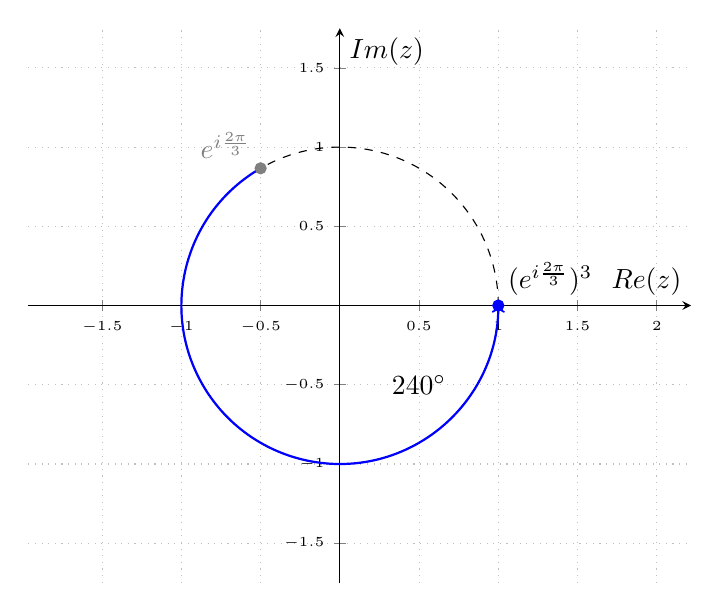
\begin{tikzpicture}
                      \begin{axis}[
                              axis equal,
                              ylabel={$\operatorname{Im}(z)$},
                              xlabel={$\operatorname{Re}(z)$},
                              xmin=-1.5, xmax=1.75,
                              ymin=-1.75, ymax=1.75,
                          ]
                          \addplot[color=gray,only marks] coordinates {(-0.5, {sqrt(3)/2})} node[above left, gray] {$e^{i\frac{2 \pi }{3}}$};
                          \draw[dashed] (0,0) circle [radius=1];
                          \draw[->,thick, blue](-0.5,{sqrt(3)/2}) arc [start angle=120, end angle=360, radius=1];
                          \node at (0.5,-0.5) {$240^\circ$};
                          \addplot[blue, only marks] coordinates {(1,0)} node[above right, black] {$(e^{i\frac{2 \pi }{3}})^3$};
                      \end{axis}
                  \end{tikzpicture}
              \end{center}

              Somit rotiert die Potenzierung mit $3$ den Punkt $e^{i\frac{2 \pi
              }{3}}$ zur $1$. Algebraisch ergibt sich dies aus der Euler'schen
              Identität: $({e^{i\frac{2 \pi }{3}}})^3 = e^{i2\pi} = 1$.

              Jede weitere Multiplikation von $e^{i2\pi}$ mit sich selbst
              resultiert somit in einer Rotation des Punktes um weitere
              $360^\circ$, was wieder in dem Punkt $1$ resultiert.

              Somit ergibt sich
              \[
                  {\left(\frac{1+i\sqrt{3}}{1-i\sqrt{3}}\right)}^{204}
                  = {(e^{i\frac{2 \pi }{3}} )}^{204}
                      = {({(e^{i\frac{2 \pi }{3}} )}^3)}^{68}
                      = {(e^{i2\pi})}^{68}
                      = 1^{68}
                  = 1.
              \]

              Um die Frage aus der Aufgabenstellung zu beantworten: Der
              Realteil von $1$ ist sicherlich $1$, der Imaginärteil ist $0$,
              der Abstand zur $0$ beträgt $1$ (Betrag), und das Argument ist
              ein Vielfaches von $2\pi$.

        \item Betrachten wir zunächst die beiden Basen der Summanden.

              Multiplizieren wir ${(1 + i)}^2$ aus erhalten wir \[
                  {(1 + i)}^2 = 1 + 2i + i^2 = 2i
              \] und für ${(1 - i)}^2$ erhalten wir \[
                  {(1 - i)}^2 = 1 - 2i + i^2 = -2i.
              \]

              Setzen wir nun wieder ein
              \[
                  (1 + i)^{2n} + (1 - i)^{2n} = {(2i)}^n + {(-2i)}^n = 2^ni^n(1+ {(-1)}^n).
              \]

              Betrachten wir soeben die folgenden fälle.

              \begin{description}
                  \item[$n$ gerade]
                        ist $1+ {(-1)}^n = 2$ und $i^n = {(-1)}^\frac{n}{2}$ also $2^ni^n(1+ {(-1)}^n) = 2^{n+1}{(-1)}^{\frac{n}{2}}$

                        Somit sehen wir das der Imaginärteil immer gleich null
                        ist. Der Betrag, Realteil hingegen hängt proportional
                        von $n$ ab also \[
                            |(1 + i)^{2n} + (1 - i)^{2n}|  = \operatorname{Re}((1 + i)^{2n} + (1 - i)^{2n}) = 2^{n+1}{(-1)}^{\frac{n}{2}}.
                        \].

                        Das Argument hingegen beträgt $\pi \frac{n}{2}$ da
                        somit $2^{n+1} e^{i\pi\frac{n}{2}} = 2^{n+1}
                        {(e^{i\pi})}^\frac{n}{2} =
                        2^{n+1}{(-1)}^{\frac{n}{2}}$.

                  \item[$n$ ungerade]
                        erhalten wir $1+ {(-1)}^n = 0$ und somit Real-, Imaginärteil sowie Betrag von $(1 + i)^{2n} + (1 - i)^{2n}$ gleich
                        null sowie Argument beliebig.
              \end{description}

              \begin{center}
                  \begin{tikzpicture}
                      \begin{axis}[
                              ylabel={$\operatorname{Im}(z)$},
                              xlabel={$\operatorname{Re}(z)$},
                              xmin=-8, xmax=8,
                          ]

                          \addplot+[font=\tiny] coordinates {(2,0)} node [above right] {$(1 + i)^{2 \cdot 0} + (1 - i)^{2 \cdot 0}$};

                          \addplot+[font=\tiny] coordinates {(0,0)} node [above left] {$(1 + i)^{2 \cdot 1} + (1 - i)^{2 \cdot 1}$};

                          \addplot+[font=\tiny] coordinates {(-8,0)} node [below right] {$(1 + i)^{2 \cdot 2} + (1 - i)^{2 \cdot 2}$};

                          \addplot+[font=\tiny] coordinates {(0,0)} node [below right] {$(1 + i)^{2 \cdot 3} + (1 - i)^{2 \cdot 3}$};
                      \end{axis}
                  \end{tikzpicture}
              \end{center}
    \end{enumerate}
\end{proof}
\end{problem}

\begin{problem}[Teilmengen der komplexen Ebene]{4 Punkte}
Skizzieren Sie die folgenden Teilmengen $A_k \subset \mathbb{C}$:
\begin{enumerate}
    \item $A_1 = \{z \in \mathbb{C}^* | \text{Re}\left(\frac{1}{z}\right) \leq 2\}$
    \item $A_2 = \{z \in \mathbb{C} | |z - 1| = \text{Re}(z)\}$
    \item $A_3 = \{z \in \mathbb{C} | \overline{z}z + z - 3\overline{z} + 1 = 0\}$
\end{enumerate}

\begin{proof}
    \leavevmode
    \begin{enumerate}
        \item Wie in Aufgabe 4 beschrieben erhalten wir für $- \frac{1}{z} =
              \frac{-a}{a^2+b^2} + i\frac{b}{a^2+b^2}$. Es ist leicht zu sehen
              das für $\frac{1}{z} = \frac{a}{a^2+b^2} + i\frac{b}{a^2+b^2}$
              erhalten also $\operatorname{Re}(\frac{1}{z}) = \frac{a}{a^2+b^2}
              \leq 2$.

              \begin{center}
                  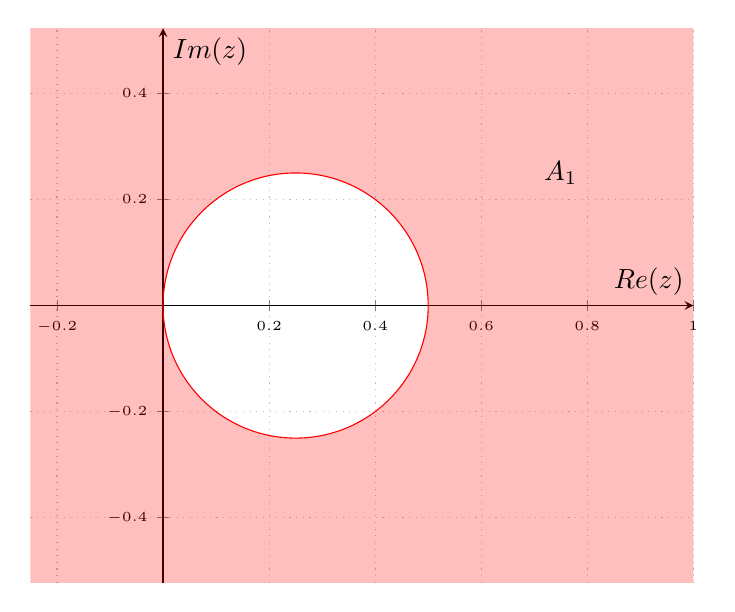
\begin{tikzpicture}
                      \begin{axis}[
                              axis equal,
                              ylabel={$\operatorname{Im}(z)$},
                              xlabel={$\operatorname{Re}(z)$},
                              xmin=-0.25, xmax=1,
                              ymin=-0.5, ymax=0.5
                          ]
                          \draw[red] (0.25,0) circle (0.25);
                          \fill[red, fill opacity=0.25] (-2,-2) rectangle (2,2) (0.25,0) circle (0.25);
                          \node at (0.75, 0.25) {$A_1$};
                      \end{axis}
                  \end{tikzpicture}
              \end{center}
        \item Für $z \in \field{C}$ mit $z := a +ib$ $a,b \in \reals$ erhalten
              wir für $|z - 1| = \operatorname{Re}(z)$
              \[
                  \sqrt{{(a-1)}^2 + b^2} = a
              \] oder \[
                  b = \pm \sqrt{2a-1}.
              \]

              \begin{center}
                  \begin{tikzpicture}
                      \begin{axis}[
                              axis equal,
                              ylabel={$\operatorname{Im}(z)$},
                              xlabel={$\operatorname{Re}(z)$},
                              xmin=-0.25, xmax=1.5,
                              ymin=-2, ymax=2,
                              smooth,
                              domain=0.5:2,
                              samples=100,
                              clip=false,
                          ]
                          \addplot+[no markers, blue] {sqrt(x^2 - (x-1)^2)} node[below right] {$A_2$};
                          \addplot+[no markers, blue] {-sqrt(x^2 - (x-1)^2)};
                      \end{axis}
                  \end{tikzpicture}
              \end{center}
        \item Setzen wir wiederum unsere definition von $z$ ein erhalten wir
              für $\overline{z}z + z - 3\overline{z} + 1 = 0$ \[
                  a^{2}+b^{2}+a+b-3(a-b) + 1 = 0
              \] oder \[
                  b = \pm \sqrt{ -a^2 +2a + 3 } - 2.
              \]

              \begin{center}
                  \begin{tikzpicture}
                      \begin{axis}[
                              axis equal,
                              ylabel={$\operatorname{Im}(z)$},
                              xlabel={$\operatorname{Re}(z)$},
                              xmin=-0.25, xmax=1.5,
                              ymin=-4.5, ymax=1.5,
                              smooth,
                              domain=-1:3,
                              samples=100,
                              clip=false,
                          ]
                          \addplot+[no markers, blue] {-2 + sqrt(3 + 2*x - x^2)} node[above right] {$A_3$};
                          \addplot+[no markers, blue] {-2 + - sqrt(3 + 2*x - x^2)} node[above right] {$A_3$};
                      \end{axis}
                  \end{tikzpicture}

              \end{center}
    \end{enumerate}
\end{proof}

\end{problem}

\begin{problem}[Gleichungen im Komplexen]{4 Punkte}
Bestimmen Sie die Lösungen der folgenden Gleichungen, und geben Sie bei b) auch numerisch approximative Werte auf fünf Stellen hinter dem Dezimalpunkt an:
\begin{enumerate}
    \item $z^5 = 4 - 4i$
    \item $\cos(z) = 2024$
\end{enumerate}
\end{problem}

\begin{problem}[Obere Halbebene]{4 Punkte}
Die obere Halbebene ist die Menge aller komplexen Zahlen mit positivem Imaginärteil: $H := \{z \in \mathbb{C} | \text{Im}(z) > 0\}$. Zeigen Sie, dass durch $T(z) := -\frac{1}{z}$ eine Bijektion $T : H \rightarrow H$ der oberen Halbebene auf sich selber gegeben ist.

\begin{proof}
    Beginnen wir zunächst zu zeigen das $\forall z \in \field{C}$ mit $\Im(z) > 0$ gilt $\Im(-\frac{1}{z}) > 0$.

    Nehmen wir $z \in \field{C}$ mit $z := a + ib$ $a,b \in \reals$, bemerke
    das $\Im(z) > 0 \Rightarrow b > 0$, somit gilt
    \[
        - \frac{1}{z} = - \frac{\bar{z}}{z\bar{z}} = - \frac{a - ib}{a^2 + b^2} = \frac{-a + ib}{a^2 + b^2} = \frac{-a}{a^2+b^2} + i\frac{b}{a^2+b^2},
    \] also $\Im(-\frac{1}{z}) = \frac{b}{a^2 + b^2}$ und $\frac{b}{a^2 + b^2}
       > 0$ da $b > 0$ und somit auch $a^2 + b^2 > 0$, somit $\Im(-\frac{1}{z})
       > 0$.

    Somit bleibt es noch zu zeigen das $T$ Injektive sowie Surjektiv ist.

    \textbf{Injektive}

    Um zu zeigen, das $T$ Injektive ist muss gezeigt werden $T(z) = T(z^\prime)
    \Rightarrow z = z^\prime$. Nehmen wir uns zwei $z, z^\prime \in H$ somit
    folgt
    \[
        - \frac{1}{z} = - \frac{1}{z^\prime} \Rightarrow -1 = \frac{-z}{z^\prime} \Rightarrow -z^\prime = -z \Rightarrow z^\prime = z.
    \]

    \textbf{Surjektiv}

    Um zu zeigen, das $T$ surjektiv ist muss gezeigt werden das $\forall z \in
    H$ ein $z^\prime$ in $H$ existiert mit $T(z^\prime) = z$. Wählen wir
    $z^\prime = - \frac{1}{z}$, wie bereits zu begin des Beweises gezeigt
    wurde, gilt $\forall z \in H$ $T(z) \in H$, somit $z^\prime \in H$, wenn
    wir nun $T$ auf $z^\prime$ an erhalten wir $T(z^\prime) =
    -\frac{1}{-\frac{1}{z}} = z$. Somit $\exists z^\prime \in H$ $\forall z \in
    H$ mit $T(z^\prime) = z$.

\end{proof}
\end{problem}

\begin{problem}[Einheitskreis]{4 Punkte}
a) Gegeben sei die Abbildung $f : \mathbb{C}^* = \mathbb{C} \setminus \{0\} \rightarrow \mathbb{C}$, $z \mapsto \frac{1}{z}$. Finden Sie eine geometrische Interpretation dieser Abbildung in der komplexen Ebene! Was geschieht durch die Abbildung anschaulich?

b) Gegeben sei eine weitere Abbildung $g : \mathbb{C}^* \rightarrow
\mathbb{C}$, $z \mapsto \frac{1}{\overline{z}}$. Verdeutlichen Sie geometrisch,
warum diese Abbildung \qouted{Inversion an der Einheitskreislinie} genannt
wird! Welche Fixpunkte ($g(z) = z$) besitzt die Abbildung g?

\begin{proof}
    \leavevmode
    \begin{enumerate}
        \item Betrachten wir zunächst was mit einem generischen Punkt $z \in
              \field{C}$ passiert, wenn wir $f$ auf $z$ anwenden.

              \[
                  f(z) = \frac{1}{z} = \frac{\bar{z}}{z \bar{z}} = \frac{\bar{z}}{{|z|}^2}
              \] also wird $z$ auf sein konjugiertes komplexes abgebilded und
                 dann durch seinen quadrierten Betrag skaliert.

              Visualisiert für einen konkreten Punkt $z = 1 + 2i$, sieht die
              transformation durch $f$ wie folgt aus.

              \begin{center}
                  \begin{tikzpicture}
                      \begin{axis}[
                              axis equal,
                              ylabel={$\operatorname{Im}(z)$},
                              xlabel={$\operatorname{Re}(z)$},
                              xtick distance=1,
                              ytick distance=1,
                              xmin=-1, xmax=2,
                              ymin=-4, ymax=4,
                          ]
                          \addplot[mark=*] coordinates {(1,2)} node[above right] {$z$};
                          \draw[dotted] (0,0) -- (1, -2) -- (1, 2);
                          \addplot[mark=*] coordinates {(1,-2)} node[below right] {$\bar{z}$};
                          \addplot[mark=*] coordinates {(0.2, -0.4)} node[below right] {$\frac{1}{z}$};
                          \draw[dashed] (0,0) circle [radius=1];
                      \end{axis}
                  \end{tikzpicture}
              \end{center}

              Somit spiegelt $f$ $z$ zunächst über die reale Zahlenebene und
              dann verschiebt sie $\bar{z}$ inverse proportional entlang seiner
              Achse.

        \item Für $g$ Betrachten wir wiederum einen generischen Punkt $z \in
              \field{C}$. \[
                  g(z) = \frac{1}{\bar{z}} = \frac{z}{\bar{z}z} = \frac{z}{{|z|}^2}
              \]

              Diese Abbildung ist relative ähnlich zu $f$ nur das hier $z$
              nicht gespiegelt wird.

              Visualisiert für einen konkreten Punkt $z = 1 + 2i$, sieht die
              transformation durch $g$ wie folgt aus.

              \begin{tikzpicture}
                  \begin{axis}[
                          axis equal,
                          ylabel={$\operatorname{Im}(z)$},
                          xlabel={$\operatorname{Re}(z)$},
                          xtick distance=1,
                          ytick distance=1,
                          xmin=-1, xmax=2,
                          ymin=-4, ymax=4,
                      ]
                      \addplot[mark=*] coordinates {(1,2)} node[above right] {$z$};
                      \addplot[mark=*] coordinates {(1,-2)} node[below right] {$\bar{z}$};
                      \draw[dotted] (0,0) -- (1, 2) -- (1, -2);
                      \addplot[mark=*] coordinates {(0.2, 0.4)} node[above right] {$\frac{1}{\bar{z}}$};
                      \draw[dashed] (0,0) circle [radius=1];
                  \end{axis}
              \end{tikzpicture}

              Betrachten wir nun die Fixpunkte $g(z) = z$ erhalten wir \[
                  z = \frac{1}{\bar{z}} \Rightarrow z \bar{z} = 1 \Rightarrow \sqrt{z \bar{z}} = 1
              \] also alle Punkte $z \in \field{C}$ mit einem Betrag von $1$
                 oder vereinfacht, alle Punkte die auf der Einheitskreislinie
                 liegen.

              Somit ergibt sich die Bezeichnung \qouted{Inversion an der
              Einheitskreislinie}, durch die eigenschaft der Funktion Punkte
              die innerhalb des Einheitskreises liegen außerhalb des
              Einheitskreises zu projizieren und Punkte außerhalb in das Innere
              des Einheitskreises. Nur die Punkte auf der Einheitskreislinie
              bleiben unberührt.

              Ich habe mir die Freiheit genommen das Ganze einmal zeichnen zu
              lassen, bitte bemerke, dass wir hier $z := a + ib$ als $a + b$
              darstellen.

              % \begin{center}
              %  \begin{tikzpicture}
              %   \begin{axis}[
              %     ylabel={$\operatorname{Im}(z)$},
              %     xlabel={$\operatorname{Re}(z)$},
              %     zlabel={$g(z)$},
              %     every axis y label/.append style={at=(ticklabel* cs:0)},
              %     every axis x label/.append style={at=(ticklabel* cs:1)},
              %     xmin=-2, xmax=2,
              %     ymin=-2, ymax=2,
              %     zmin=-2, zmax=2,
              %    ]
              %    \addplot3[
              %     surf,
              %     colormap/cool,
              %     samples=50,
              %     domain=-2:2,
              %     y domain=-2:2,
              %    ] {(x+y)/(x^2+y^2)};
              %   \end{axis}
              %  \end{tikzpicture}
              % \end{center}

    \end{enumerate}
\end{proof}
\end{problem}

\begin{problem}[Simple Gleichung, komplexe Lösungen?]{4 Sonderpunkte}
Bestimmen Sie (mit Beweis) alle komplexen Lösungen $z \in \mathbb{C}$ der Gleichung $\text{Im}(z) = 2\sin(z)\cos(z)$.
\end{problem}

\end{document}
